\documentclass[9pt]{article}

\usepackage{graphicx, xcolor, amssymb} % Required for inserting images
\usepackage{amsmath}
\usepackage{amsfonts}
\usepackage{ctex}
\usepackage{enumitem}
\usepackage{longtable}
\usepackage{makecell} % 换行

% 使用分栏宏包
\usepackage{multicol} 
\usepackage{multirow}
\setlength{\columnseprule}{0.4pt} % 分割线

% 设置字体
\usepackage{unicode-math}
\setmainfont{Cambria}
\setmathfont{Cambria Math}

% 调整页面布局
\usepackage[a4paper, top=0.7cm, bottom=1cm, left=0.7cm, right=.7cm]{geometry}
\setlength{\footskip}{15pt}

% 设置页脚/页眉
\usepackage{fancyhdr}
\fancyfoot[C]{Copyright By Jingren Zhou | Page \thepage}
\fancyhead[]{}
\pagestyle{fancy}
% 去除线
\renewcommand{\headrulewidth}{0pt}
\renewcommand{\footrulewidth}{0pt}

% 设置 section/subsection 之间的行间距
\usepackage{titlesec}
\titlespacing*{\section}{0pt}{0pt}{0pt}
\titlespacing*{\subsection}{0pt}{0pt}{0pt}

% 调整标题上下间距
\usepackage{titling}
\setlength{\droptitle}{-2.4cm} % 负值表示向上移动

% 设置标题,作者,时间
\title{LPMS Note}
\author{}
\date{}

% 正文
\begin{document}


% 标题
\maketitle
\thispagestyle{fancy}
\vspace{-3.5cm}

% 字体大小
\fontsize{10pt}{11pt}\selectfont
\setlength{\parindent}{8pt}

\section{Definition of LP and General LP} % Definition of LP and General LP

\subsection{Definition of LP}

\textbf{Linear Programming (LP)}: {\small Let \ \ $x_i$: \textbf{Decision Variables} \quad $a_{ij},b_i,c_i$: \textbf{parameters} \quad $f$: \textbf{Objective Function} \quad} {\scriptsize\textbf{Constraints}: subject 后的限制条件}

\vspace{-9pt}
\begin{multicols}{2}

    LP problem can be written as:
    \[
    \begin{aligned}
        \text{maximize} \quad \ \ f = & c_1x_1 + c_2x_2 + \cdots + c_nx_n & \\
        \text{subject to} \quad \qquad & a_{11}x_1 + a_{12}x_2 + \cdots + a_{1n}x_n \leq b_1 & \\
                                & a_{21}x_1 + a_{22}x_2 + \cdots + a_{2n}x_n \leq b_2 & \\
                                & \vdots & \\
                                & a_{m1}x_1 + a_{m2}x_2 + \cdots + a_{mn}x_n \leq b_m & \\
                                & x_1 \geq 0, x_2 \geq 0, \cdots, x_n \geq 0 &
    \end{aligned}
    \]
    
    \columnbreak

    We can also write the LP problem in matrix form:

    \vspace{5pt}
    $
    A=
    \begin{pmatrix}
        a_{11} & \cdots & a_{1n} \\
        \vdots & \ddots & \vdots \\
        a_{m1} & \cdots & a_{mn} \\
    \end{pmatrix}
    ,\mathbf{b}=
    \begin{pmatrix}
        b_1 \\
        \vdots \\
        b_m
    \end{pmatrix}
    ,\mathbf{c}=
    \begin{pmatrix}
        c_1 \\
        \vdots \\
        c_n
    \end{pmatrix}
    ,\mathbf{x}=
    \begin{pmatrix}
        x_1 \\
        \vdots \\
        x_n
    \end{pmatrix}
    $

    \[
    \begin{aligned}
        \text{maximize} \quad \ \ f = & \mathbf{c}^T\mathbf{x} & \\
        \text{subject to} \quad \qquad & A\mathbf{x} \leq \mathbf{b} & \mathbf{x} \geq 0 \\
    \end{aligned}
    \]
\end{multicols}
\vspace{-9pt}

At this time, we have the following definitions:

\begin{enumerate}[itemsep=-2pt, topsep=-2pt]
    \item \textbf{Feasible Solution}: 可行解, 满足所有约束条件的解. (i.e. $A\mathbf{x}\leq\mathbf{b}$)
    \item \textbf{Optimal Solution}: 最优解 (可多个)
    \item \textbf{Feasible Region}: 可行域, 所有可行解的集合.
\end{enumerate}

\textbf{Find Optimal Solution}: \textbf{Graphical Method} \quad or \quad \textbf{Simplex Method}


\subsection{General LP Problem}

\textbf{Slack Variables}: 对每个不等式约束, 各引入(Slack Variables) $x_i$ ($i>n$) 来将其转化为\textit{等式}约束. (i.e. $A\mathbf{x}\leq\mathbf{b}$ $\Rightarrow$ $\overline{A}\mathbf{x}=\mathbf{b}$)

\vspace{-9pt}
\begin{multicols}{2}

    LP problem can be written as: \quad \quad ps: $x_{i}\geq0$ ($i>n$).
    \[
    \begin{aligned}
        \text{maximize} \quad \ \ f = & c_1x_1 + c_2x_2 + \cdots + c_nx_n & \\
        \text{subject to} \quad \qquad & a_{11}x_1 + a_{12}x_2 + \cdots + a_{1n}x_n + \textcolor{red}{x_{n+1}} = b_1 & \\
                                & a_{21}x_1 + a_{22}x_2 + \cdots + a_{2n}x_n + \textcolor{red}{x_{n+2}} = b_2 & \\
                                & \vdots & \\
                                & a_{m1}x_1 + a_{m2}x_2 + \cdots + a_{mn}x_n + \textcolor{red}{x_{n+m}} = b_m & \\
                                & x_1 \geq 0, x_2 \geq 0, \cdots, x_{n+m} \geq 0 &
    \end{aligned}
    \]
    
    \columnbreak

    We can also write the LP problem in matrix form:

    \vspace{5pt}
    $
    \overline{A}= [ \ A  \ \ I_m \ ]
    ,\mathbf{b}=\mathbf{b}
    ,\overline{\mathbf{c}}=
    \begin{pmatrix}
        \mathbf{c} \\
        \mathbf{0}_{ m\times 1}
    \end{pmatrix}
    ,\mathbf{x}=
    \begin{pmatrix}
        \mathbf{x} \\
        \vdots \\
        x_{n+m}
    \end{pmatrix}
    $

    \[
    \begin{aligned}
        \text{maximize} \quad \ \ f = & \overline{\mathbf{c}}^T\mathbf{x} & \\
        \text{subject to} \quad \qquad & \overline{A}\mathbf{x} = \mathbf{b} & \mathbf{x} \geq 0 \\
    \end{aligned}
    \]

\end{multicols}
\vspace{-5pt}

\fbox{\parbox[c]{0.98\textwidth}{
At this time, we have the following definitions:

\begin{enumerate}[itemsep=-2pt, topsep=-2pt]
    \item \textbf{Basic Solution}: Solution of $\overline{A}\mathbf{x}=\mathbf{b}$. \ \ $\rightarrow$ \ \ 得到: $\mathbf{x}_B,\quad \mathbf{x_N}=0${\scriptsize (要求)} \quad (不一定$\mathbf{x}\geq\mathbf{0}$, \quad $\mathbf{x}_B$不一定$\geq0$) \\
    {\scriptsize ps: 只有 把某一组 $m$ 个线性无关列选为基,令其余变量固定为 $0$ 后求得的那一个唯一向量 才叫 Basic Solution}
    \item \textbf{Basic Feasible Solution (BFS)}: If a Basic Solution $\mathbf{x}_B,\mathbf{x_N=0}$ have: $\mathbf{x}_B\geq0$, then $\mathbf{x}$ is a Basic Feasible Solution.
    \item {\small \textbf{Basic Variables}: $\mathbf{x}_B$ \quad \textbf{Nonbasic Variables}: $\mathbf{x}_N$ \quad \textbf{Basic Matrix}: $B$ \quad \textbf{Nonbasic Matrix}: $N$ \quad \textbf{Basic Index}: $\mathcal{B}$ \quad \textbf{Nonbasic Index}: $\mathcal{N}$} \\
    {\scriptsize ps: 均为人为规定 $\mathcal{B}$ 和 $\mathcal{N}$ 后得到.}
\end{enumerate}
}}

\fbox{\parbox[c]{0.98\textwidth}{
For the LP problem, we consider the following:

\begin{enumerate}[itemsep=-2pt, topsep=-2pt]
    \item \textbf{Convex Set}: Set $K$ is convex if, for any two points $\mathbf{x},\mathbf{x'}\in K$, the line segment $\mathbf{x}_\theta=\theta\mathbf{x}+(1-\theta)\mathbf{x'}$ for $\theta\in[0,1]$ is also in $K$.
    \item \textbf{Vertex of a Convex Set}: A vertex of a convex set $K$ is a point $\mathbf{x}\in K$ such that it does not lie strictly within any line segment joining two points in $K$. \qquad ({\scriptsize ps: there are $\frac{(m+n)!}{m!n!}$ vertices for LP problem})
    \item \textbf{Theorem I}: If LP has a unique optimal solution, then it is a vertex. \qquad \textcolor{red}{(optimal $\leftrightarrow$ vertex)}
    \item \textbf{Theorem II}: If LP has a non-unique solution, $\exists$ optimal solution at vertex. \qquad \textcolor{red}{(optimal $\leftrightarrow$ vertex)}
\end{enumerate}

\textbf{Remark}: \textcolor{red}{BFS and Vertices are NOT 1-1} (与它是否是唯一optimal solution 无关!) \\ \star \ Happened if one of \textit{basic variables} of \textit{optimal solution} is zero. $\rightarrow$ Referred as \textbf{degenerate}.
}}


\section{Simplex Method} % Simplex Method

\subsection{Some Definitions}

For LP problem: max $f=\mathbf{c}^T\mathbf{x}$ \quad s.t. $A\mathbf{x}\le\mathbf{b}$ \quad $\mathbf{x}\geq0$

By adding slack variables, we can write it as: max $f=\overline{\mathbf{c}}^T\mathbf{x}$ \quad s.t. $\overline{A}\mathbf{x}=\mathbf{b}$ \quad $\mathbf{x}\geq0$

\fbox{\parbox[c]{0.98\textwidth}{
\begin{enumerate}[itemsep=-2pt, topsep=-2pt]
    \item \textbf{We can define Index}: $\mathcal{B},\mathcal{N}$
    \item \textbf{Basic Matrix}: $B$ (整个 $\overline{A}$ 中在 index $\mathcal{B}$ 中的列) \quad \textbf{Nonbasic Matrix}: $N$ (整个 $\overline{A}$ 中在 index $\mathcal{N}$ 中的列) \quad \textcolor{red}{$\overline{A}\rightarrow[B \ N]$}
    \item \textbf{Basic Variables}: $\mathbf{x}_B$ (对应 $B$ 列因有的变量) \quad \textbf{Nonbasic Variables}: $\mathbf{x}_N$ (对应 $N$ 列因有的变量) \quad {\scriptsize \textcolor{red}{$\mathbf{x}\to\begin{pmatrix}\mathbf{x}_B \\ \mathbf{x}_N\end{pmatrix}$}}
    \vspace{-5pt}
    \item \textbf{Matrix Cost}: $\mathbf{c}_B$ ($f$中对应 $\mathbf{B}$ 变量的系数) \quad \textbf{Nonbasic Cost}: $\mathbf{c}_N$ ($f$中对应 $\mathbf{N}$ 变量的系数) \quad {\scriptsize \textcolor{red}{$\overline{\mathbf{c}}\rightarrow\begin{pmatrix}\mathbf{c}_B \\ \mathbf{c}_N\end{pmatrix}$}}
    \vspace{-5pt}
    \item \textbf{Other}: \textcolor{red}{$\overline{A}\mathbf{x}=\mathbf{b}\Leftrightarrow B\mathbf{x}_B+N\mathbf{x}_N=\mathbf{b}$} \quad || \quad Let \textcolor{red}{$\widehat{\mathbf{b}}=B^{-1}\mathbf{b}$ \quad $\widehat{N}=B^{-1}N$} \quad || \quad Thus \textcolor{red}{$\mathbf{x}_B=\widehat{\mathbf{b}}-\widehat{N}\mathbf{x}_N$}
    \item \textbf{Objective Value}: \textcolor{red}{$f=\overline{\mathbf{c}}^T\mathbf{x}=\mathbf{c}_B^T\mathbf{x}_B+\mathbf{c}_N^T\mathbf{x}_N=\widehat{f}+\widehat{c}^T_N\mathbf{x}_N$} \qquad where \textcolor{red}{$\widehat{f}=\mathbf{c}^T_B\widehat{b}$ \quad $\widehat{\mathbf{c}}_N=\mathbf{c}_N-\widehat{N}\mathbf{c}_B=\mathbf{c}_N-N^TB^{-T}\mathbf{c}_B$}
\end{enumerate}
}}

\star \ {\small \textbf{Remark}: For \textit{Basic Solution}, we let $\mathbf{x_B}=\widehat{\mathbf{b}}$ and $\mathbf{x_N}=\mathbf{0}$. \qquad \textbf{Remark}: If basic Solution have $\widehat{\mathbf{b}}\geq0$, it is a \textbf{Basic Feasible Solution (BFS)}.}

\star \ {\small \textcolor{red}{\textbf{Theorem}: If BFS have: $\widehat{\mathbf{c}}_N\leq0$, it is an \textbf{Optimal Solution}}}

\newpage


\subsection{Simplex Algorithm}

\fbox{\parbox[c]{0.98\textwidth}{
\textbf{An Initial BFS}: Try $\mathcal{B}=\{n+1,...,n+m\}$ and $\mathcal{N}=\{1,...,n\}$ \ \ $\Rightarrow$ \ \ $B=I,N=A$ , $\mathbf{x}_B=\widehat{\mathbf{b}}=\mathbf{b}$, $\mathbf{x}_N=\mathbf{0}$, $\mathbf{c}_B=\mathbf{0}$, $\mathbf{c}_N=\mathbf{c}$

\qquad \textbf{Corollary}: If $\widehat{\mathbf{b}}=\mathbf{b}\geq0$, it's a BFS.
}}


\fbox{\parbox[c]{0.98\textwidth}{
\textbf{Simplex Algorithm}:

\begin{enumerate}[itemsep=-2pt, topsep=-2pt]
    \item If \textbf{An Initial BFS} is BFS$\to$\ref{simplex.2} \quad || \quad If we have an BFS$\to$\ref{simplex.2} \quad || \quad Else: Go to \textbf{Phase I Problem}
    \item\label{simplex.2} If $\widehat{\mathbf{c}}_N\leq0. \Rightarrow$ Optimal Solution \quad || \quad Else: Go to \ref{simplex.3}
    \item\label{simplex.3} Let $q\in$ (local index in $N$) \ \ ; \ \ $q'\in \mathcal{N}$ (global index) \quad || \quad $\widehat{c}_i:=\widehat{\mathbf{c}}_N$中第i个分量($\widehat{c}_i:=\widehat{\mathbf{c}}_N^T\mathbf{e}_i$) \quad || \quad such that: 
    
    $\widehat{c}_q=\widehat{\mathbf{c}}_N$中最大的正的分量 {\scriptsize ($c_q=\arg\max_{i=1,...,n \ ; \ c_i>0} \widehat{c}_i$)} \quad ; \quad $q'$ is the index corresponding to $q$ in $\mathcal{N}$ {\footnotesize (对应的在$\mathcal{N}$的index(global index))}
    
    Thus, we find $q,q'$ \qquad Go to \ref{simplex.4}

    \item\label{simplex.4} Let $p\in$ (local index in $B$) \ \ ; \ \ $p'\in\mathcal{B}$ (global index) \quad || \quad \textcolor{red}{$\mathbf{a}_q:=N$中的第q列}($\mathbf{a}_q=N\mathbf{e}_q$) \quad || \quad Let \textcolor{red}{$\widehat{\mathbf{a}_q}=B^{-1}\mathbf{a_q}$}:
    
    If $\widehat{\mathbf{a}_q}\leq0$ \ \ $\Rightarrow$ \ \ LP is unbounded. \quad || \quad Else: LP is bounded$\to$\ref{simplex.5}
    
    \item\label{simplex.5} Let \textcolor{red}{$p=\arg\min_{i=1,...,m \ ; \ \widehat{a}_{iq}>0}\frac{\widehat{b_i}}{\widehat{a}_{iq}}$} {\scriptsize $p$是对应的 local index,not value, \star 用$\overline{\alpha}=\frac{\widehat{b_p}}{\widehat{a}_{pq}}$代表值} \qquad {\scriptsize $\widehat{b_i}$ 代表$\widehat{\mathbf{b}}$的第$i$个分量; \quad $\widehat{a}_{iq}$ 代表 $\widehat{\mathbf{a}_q}$的第$i$个分量}
    
    Let $p'$ \ be (global) index corresponding to $p$.
    
    Thus, we find $p,p'$ \qquad Go to \ref{simplex.6}

    \item\label{simplex.6} Exchange $p'$ and $q'$ between $\mathcal{B}$ and $\mathcal{N}$ \ \ $\Rightarrow$ \qquad Update $\mathcal{B},\mathcal{N},B,N,\widehat{\mathbf{b}},...$ \quad {\scriptsize ps: \textcolor{red}{New $B := B + (a_q - B e_p) e_p^T$}}
    \item Calculate $\widehat{\mathbf{c}}_N$. Go to \ref{simplex.2}
\end{enumerate}
}}

\textcolor{red}{\textbf{Remark}}: If we consider using $\mathbf{x}+\alpha\mathbf{d}$ where $\mathbf{d}\to[\mathbf{d}_B \ \mathbf{d}_N]^T$; $\mathbf{d}_N=\mathbf{e}_q$ $\mathbf{d}_B=-\widehat{\mathbf{a}}_q$, then:

We have: {\scriptsize $\begin{pmatrix}\mathbf{x}_B \\ \mathbf{x}_N\end{pmatrix}=\begin{pmatrix}\widehat{\mathbf{b}} \\ 0\end{pmatrix}+\alpha\begin{pmatrix}-\widehat{\mathbf{a}}_q \\ \mathbf{e}_q\end{pmatrix}$} and $f=\mathbf{c}^T_B\mathbf{x}_B+\mathbf{c}^T_N\mathbf{x}_N=\mathbf{c}^T_B(\widehat{\mathbf{b}}-\alpha\widehat{\mathbf{a}}_q)+\mathbf{c}^T_N(\alpha\mathbf{e}_q)=\widehat{f}-\alpha(\mathbf{c}^T_N\mathbf{e}_q-\mathbf{c}_B^TB^{-1}N\mathbf{e}_q)=\widehat{f}+\alpha\widehat{\mathbf{c}}_N\mathbf{e}_q=\widehat{f}+\alpha\widehat{c}_q$


\fbox{\parbox[c]{0.98\textwidth}{

\textbf{Phase I Problem}: (If $\mathbf{b}\ngeq0$ \& No BFS)
\begin{enumerate}[itemsep=-2pt, topsep=-2pt]
    \item Subtract \textbf{artificial variables} $x_{n+m+1},...,x_{n+m+m}\geq0$ and change objective function $f$ to: \\    
    {\centering 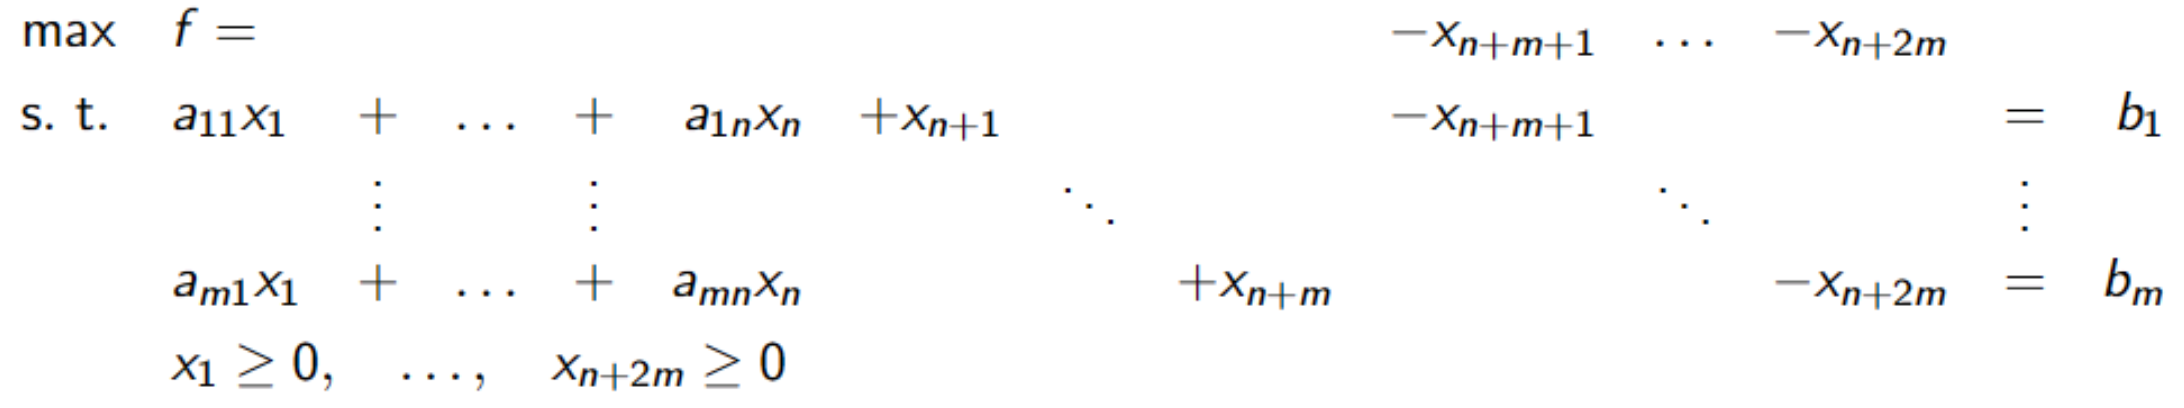
\includegraphics[width=0.6\textwidth]{formula.png}}
    \item Let $b_i:=\mathbf{b}$ 的第i个分量. (i.e. $b_i=\mathbf{b}^T\mathbf{e}_i$)
    
    Case I: $b_i\ge0$: $x_{n+i}=b_i$ is a Basic Variables. \quad and $x_{n+m+i}=0$ is a Nonbasic Variables.

    Case II: $b_i<0$: $x_{n+m+i}=-b_i$ is a Basic Variables. \quad and $x_{n+i}=0$ is a Nonbasic Variables.
    
    Other: We put $x_1,...,x_n$ as Nonbasic Variables.

    Thus we can find $\mathcal{B},\mathcal{N},B,N,\mathbf{x}_B=\widehat{\mathbf{b}}=B^{-1}\mathbf{b}=|\mathbf{b}|,\mathbf{x}_N=\mathbf{0},\mathbf{c}_B,\mathbf{c}_N$

    \item Let \textbf{Size of Infeasibility}: is $\sum^m_{i=1}x_{n+m+i}$ \qquad $f=-\sum^m_{i=1}x_{n+m+i}\leq0$
    
    \item Consider this modified LP problem, by using Simplex Algorithm, we can find an optimal solution $\mathbf{x}$ and the value of $f$.
    
    ps: 使用刚刚我们选好的$\mathcal{B},\mathcal{N}$ 作为初始的BFS.
    \item Case I: If $f=0$ (\textcolor{red}{等价于 artificial variables都是Nonbasic Variables}), $\mathbf{x}$ is a BFS for the original LP problem. (去除artificial variables,并回到原问题(也叫Phase II Problem))
    
    Case II: \textbf{If $f<0$}: LP is infeasible (\textcolor{red}{等价于存在artificial variables是Basic Variables}).
\end{enumerate}
}}


\section{Degeneracy | Termination | Cycling | Sparsity}

\subsection{Degeneracy \& Termination}

\textcolor{red}{\textbf{Degeneracy}: If $\widehat{\mathbf{b}}$ has any zero component, then $\mathbf{x}$ is a \textbf{degenerate vertex}. (等价于$\widehat{\mathbf{b}}>0$)}

\begin{enumerate}[itemsep=-2pt, topsep=-2pt]
    \item If a point is \textit{degenerate}, then there may be multiple \textit{BFS} at that point.
    \item \star \ If $\widehat{b}_p=0$, then $\overline{\alpha}=0$, simplex algorithm may not terminate. \\ {\scriptsize ps:对于simplex algorithm 我们依靠$\widehat{\mathbf{a}}_q$中大于0的元素来决定下一个要交换的变量, 但是如果$\widehat{b}_p=0$, 那么$\overline{\alpha}=0$, 可能会导致我们在这个点上循环}
\end{enumerate}

\textcolor{red}{\textbf{Termination of Simplex Algorithm in the absence of degeneracy}: If no degenerate situation, then Simplex Algorithm will terminate in a finite number of steps.}


\fbox{\parbox[c]{0.98\textwidth}{
\textbf{Examples}: 1.The worst case of Simplex Algorithm. \ \ 2. Cyclic case of Simplex Algorithm.

\begin{enumerate}[itemsep=-2pt, topsep=-2pt]
    \item \textbf{Klee-Minty Problem}: max $f=\sum^n_{j=1}10^{j-1}x_j$ \quad ; \quad s.t. $x_i+2\sum^n_{j=i+1}10^{j-i}x_j\leq100^{n-i}$ for $i=1,...,n$ \quad ; \quad $x_i\geq0$ \\
    has $2^n$ vertices. \quad \textbf{Worst Case}: $2^n-1$ iterations.
    \item \textbf{Hall-McKinnon Problem}: max $f=x_1-5.5x_2+0.75x_3-5.75x_4$ \quad ; \quad {\scriptsize s.t.} {\tiny $2.5x-19.5x_2-3.5x_3+19.5x_4+x_5=0$ ; $0.5x_1-3.5x_2-0.5x_3+3.5x_4+x_6=0$ ; $x_i\geq0$}
\end{enumerate}
}}

\newpage


\subsection{Sparsity LP Problem}

\fbox{\parbox[c]{0.98\textwidth}{
\textbf{Implementation}: 计算/编程中的计算化简 \qquad Consider: $\widehat{\mathbf{b}}=B^{-1}\mathbf{b}$ \ \ $\widehat{\mathbf{c}}_N=\mathbf{c}_N-N^TB^{-T}\mathbf{c}_B$ \ \ $\widehat{\mathbf{a}}_q=B^{-1}\mathbf{a}_q$

\begin{enumerate}[itemsep=-2pt, topsep=-2pt]
    \item Solve: \( B \widehat{\mathbf{b}} = \mathbf{b} \) \quad to get: \(\widehat{\mathbf{b}} = B^{-1}\mathbf{b}\)
    \item Solve: \( B^T \pi = \mathbf{c}_B \) \quad to get: \(\pi = B^{-T}\mathbf{c}_B\)
    \item Solve: \(\widehat{\mathbf{c}}_N = \mathbf{c}_N - N^T\pi\) \quad to get: \(\widehat{\mathbf{c}}_N = c_N - N^TB^{-T}\mathbf{c}_B\)
    \item Solve: \( B^T \widehat{\mathbf{a}}_q = \mathbf{a}_q \) \quad to get: \(\widehat{\mathbf{a}}_q = B^{-T}\mathbf{a}_q\)
    \item Matrix $B$ is \textbf{sparse} and \textbf{invertible}. And in Simplex Algorithm, the next matrix $B$ obtained by $B := B + (a_q - B e_p) e_p^T$
\end{enumerate}
}}

\textbf{Sparse LP Problem}: For LP problem: max $f=\mathbf{c}^T\mathbf{x}$ \quad s.t. $A\mathbf{x}=\mathbf{b}$ \quad $\mathbf{x}\geq0$

\qquad It is \textbf{sparse} if the matrix $A$ is sparse. (i.e. Most of the elements of $A$ are zero)

\textbf{Find Inverse of $B$}: Decomposition $B$ into $LU$ where $L$ is lower triangular and $U$ is upper triangular.

\quad Then we can \textcolor{red}{solve $B\mathbf{x}=\mathbf{b}$ by solving $^1$ $L\mathbf{y}=\mathbf{b}$ and $^2$ $U\mathbf{x}=\mathbf{y}$}

\vspace{-5pt}
{\scriptsize 
\[
\begin{bmatrix}
a_{11} & a_{12} & a_{13} & a_{14} \\
a_{21} & a_{22} & a_{23} & a_{24} \\
a_{31} & a_{32} & a_{33} & a_{34} \\
a_{41} & a_{42} & a_{43} & a_{44} 
\end{bmatrix}
=
\begin{bmatrix}
1 & 0 & 0 & 0 \\
l_{21} & 1 & 0 & 0 \\
l_{31} & l_{32} & 1 & 0 \\
l_{41} & l_{42} & l_{43} & 1
\end{bmatrix}
\begin{bmatrix}
u_{11} & u_{12} & u_{13} & u_{14} \\
0 & u_{22} & u_{23} & u_{24} \\
0 & 0 & u_{33} & u_{34} \\
0 & 0 & 0 & u_{44}
\end{bmatrix}
=
\begin{bmatrix}
\textcolor{red}{u_{11}} & \textcolor{red}{u_{12}} & \textcolor{red}{u_{13}} & \textcolor{red}{u_{14}} \\
\textcolor{orange}{l_{21} u_{11}} & \textcolor{olive}{l_{21} u_{12} + u_{22}} & \textcolor{olive}{l_{21} u_{13} + u_{23}} & \textcolor{olive}{l_{21} u_{14} + u_{24}} \\
\textcolor{orange}{l_{31} u_{11}} & \textcolor{green}{l_{31} u_{12} + l_{32} u_{22}} & \textcolor{blue}{l_{31} u_{13} + l_{32} u_{23} + u_{33}} & \textcolor{blue}{l_{31} u_{14} + l_{32} u_{24} + u_{34}} \\
\textcolor{orange}{l_{41} u_{11}} & \textcolor{green}{l_{41} u_{12} + l_{42} u_{22}} & \textcolor{black}{l_{41} u_{13} + l_{42} u_{23} + l_{43} u_{33}} & \textcolor{purple}{l_{41} u_{14} + l_{42} u_{24} + l_{43} u_{34} + u_{44}}
\end{bmatrix}
\]
}
\vspace{-5pt}

\quad By Solving $\textcolor{red}{\blacksquare} \to \textcolor{orange}{\blacksquare} \to \textcolor{olive}{\blacksquare} \to \textcolor{green}{\blacksquare} \to \textcolor{blue}{\blacksquare} \to \textcolor{black}{\blacksquare} \to \textcolor{purple}{\blacksquare}  $


\section{Sensitive Analysis} % Sensitive Analysis

\subsection{RHS Sensitivity {\scriptsize Consider \textcolor{red}{$b_i\to b_i+\delta$}}}

\textbf{RHS Sensitivity}: $\max f=\mathbf{c}^T\mathbf{x}$ s.t. $A\mathbf{x}\leq \mathbf{b},\mathbf{x}\geq0$ \quad $\Rightarrow$ \quad $\max f=\overline{\mathbf{c}}^T\mathbf{x}$ s.t. $\overline{A}\mathbf{x}=\mathbf{b},\mathbf{x}\geq0$

\qquad ps: Assume $\mathcal{B},\mathcal{N},B,N$ yield an \textit{optimal solution}, with $\mathbf{x}_B=\widehat{\mathbf{b}},\mathbf{x}_N=\mathbf{0}$

\fbox{\parbox[c]{0.98\textwidth}{
\qquad Then, the new optimal values is: \quad \textcolor{red}{$\mathbf{x}_B=B^{-1}(\mathbf{b}+\delta \mathbf{e}_i)=\widehat{\mathbf{b}}+\delta B^{-1}\mathbf{e}_i$} \quad if $\mathbf{x}_B\geq0$

\qquad With \textcolor{red}{range of $\delta\in[ \ \underline{\delta} \ , \ \overline{\delta} \ ]$ \quad $\underline{\delta}=\max\limits_{[B^{-1}]_{ji}>0}-\frac{\widehat{b}_j}{[B^{-1}]_{ji}}$ \quad $\overline{\delta}=\min\limits_{[B^{-1}]_{ji}<0}-\frac{\widehat{b}_j}{[B^{-1}]_{ji}}$}
}}

\fbox{\parbox[c]{0.98\textwidth}{
\textbf{Fair Prices}: The objective function: \textcolor{red}{$f=\mathbf{c}^T_B\mathbf{x}_B=\mathbf{c}^T_B(\mathbf{\widehat{b}}+\delta B^{-1}\mathbf{e}_i)=\widehat{f}+\delta\pi_i$} \quad where $\widehat{f}=\mathbf{c}_B^T\widehat{\mathbf{b}}$ \quad \textcolor{red}{$\pi_i=\mathbf{c}_B^TB^{-1}\mathbf{e}_i$ (fair price)}

\begin{enumerate}[itemsep=-2pt, topsep=-2pt]
    \item \textbf{If \textit{price of unit amount} $> \ \pi_i$}: Buying more of the resource is \textit{unattractive}.
    \item \textbf{If \textit{price of unit amount} $< \ \pi_i$}: Buying more of the resource is \textit{attractive}.
    \item \textbf{For Basic Slack}: If $n+i\in\mathcal{B}$ (slack variable $x_{n+i}$ 是basic slack) \ \ $\rightarrow$ \ \ $\pi_i=0$ \qquad {\tiny (Proof: \textcolor{red}{$\pi_i=(B^{-T}\mathbf{c}_B)^T\mathbf{e}_i=\mathbf{c}_B^TB^{-1}\mathbf{e}_i$}$=0$)}
    \item \textbf{For Nonbasic Slack}: If $n+i\in\mathcal{N}$ (slack variable $x_{n+i}$ 是nonbasic slack) \ \ $\rightarrow$ \ \ $\pi_i=-\widehat{c_i}$ \\ {\tiny (Proof: Assume $n+i\in\mathcal{N}$ 在 $N$ 中的 (local) index 为 $j$. Since \textcolor{red}{$\widehat{c}_j=[\mathbf{c}_N]_j-[N]^T_j\pi$}, $[\mathbf{c}_N]_j=0$, $[N]^T_j=\mathbf{e}_i$; we have: $\pi_i=-\widehat{c_i}$)}
\end{enumerate}
}}

\qquad $\star$ Range of $\delta$ is \textit{lower|upper bound Sensitivity}

\qquad $\star$ \textit{Feasible Region} increases when $\overline{\delta}$ increases and $\underline{\delta}$ decreases.


\subsection{Cost and Coefficient Sensitivity {\scriptsize Consider \textcolor{red}{$c_i\to c_i+\delta$} \& \textcolor{red}{$a_{ij}\to a_{ij}+\delta$}}}

\textbf{Cost Sensitivity}: 即$c_i\to c_i+\delta$. \quad $\max f=\mathbf{c}^T\mathbf{x}$ subject to $A\mathbf{x}\leq \mathbf{b},\mathbf{x}\geq0$

\begin{enumerate}[itemsep=-2pt, topsep=-2pt]
    \item 小范围的变化不会改变最优解. {\scriptsize (If an LP cost coefficient is changed by a small amount, the optimal solution will not change.)}
    \item 如果$c_i\to c_i+\delta$ 对应的$i$变量在$\mathcal{B}$中(basic variables), 那么 all reduced costs will change.
    \item 如果$c_i\to c_i+\delta$ 对应的$i$变量在$\mathcal{N}$中(nonbasic variables), 那么 only the reduced cost of \textit{that} variables will change.
\end{enumerate}

\textbf{Coefficient Sensitivity}: 即$a_{ij}\to a_{ij}+\delta$. \quad $\max f=\mathbf{c}^T\mathbf{x}$ subject to $A\mathbf{x}\leq \mathbf{b},\mathbf{x}\geq0$

\begin{enumerate}[itemsep=-2pt, topsep=-2pt]
    \item 如果影响的变量在$\mathcal{B}$中(basic variables): $B$ may become singular, the optimal solution may change, etc.
    \item 如果影响的变量在$\mathcal{N}$中(nonbasic variables): One \textit{reduced cost} will change, $N$ will change.
\end{enumerate}


\section{Duality} % Duality

\fbox{\parbox[c]{0.98\textwidth}{
\textbf{Duality}: For LP problem: \textcolor{red}{max $f=\mathbf{c}^T\mathbf{x}$ \quad s.t. $A\mathbf{x}\leq \mathbf{b}, \quad\mathbf{x}\geq0$} \quad \textbf{Primal} problem \qquad $(P)$

\qquad \ \ The \textbf{dual} problem is: \textcolor{red}{min $f=\mathbf{b}^T\mathbf{y}$ \quad s.t. $A^T\mathbf{y}\geq \mathbf{c}, \quad\mathbf{y}\geq0$} \quad \textbf{Dual} problem \qquad $(D)$

\qquad \ \ - It is \textit{equivalence} to: max $f=-\mathbf{b}^T\mathbf{y}$ \quad s.t. $-A^T\mathbf{y}\leq -\mathbf{c}, \quad\mathbf{y}\geq0$

\qquad \ \ The \textbf{dual} of $(D)$ is: \textcolor{red}{min $f=-\mathbf{c}^T\mathbf{z}$ \quad s.t. $(-A^T)^T\mathbf{z}\geq (-\mathbf{b}), \ \ (\text{i.e.} \ -A\mathbf{z}\geq -\mathbf{b})$, $\quad\mathbf{z}\geq0$}

\qquad \ \ - It is \textit{equivalence} to: max $f=\mathbf{c}^T\mathbf{z}$ \quad s.t. $A\mathbf{z}\leq \mathbf{b}, \quad\mathbf{z}\geq0$, which is the \textbf{Primal} problem $(P)$.
}}

\fbox{\parbox[c]{0.98\textwidth}{
\textbf{Weak Duality Theorem}: If $\mathbf{x}$ is feasible for $(P)$ and $\mathbf{y}$ is feasible for $(D)$, then \textcolor{red}{$\mathbf{c}^T\mathbf{x}\leq\mathbf{b}^T\mathbf{y}$}.

\quad \textbf{Corollary}: If $(P)$ is unbounded \ \ $\Rightarrow$ \ \ $(D)$ is infeasible. \quad || \quad If $(D)$ is unbounded \ \ $\Rightarrow$ \ \ $(P)$ is infeasible.

\textbf{Strong Duality Theorem}: If $\mathbf{x}^*$ is optimal (basic) solution for $(P)$, then:

\qquad \textcolor{red}{$\mathbf{y}^*=\pi=B^{-T}\mathbf{c}_B$} is optimal solution for $(D)$, \quad and $\mathbf{c}^T\mathbf{x}^*=\mathbf{b}^T\mathbf{y}^*$.
}}

\newpage

\textbf{Application}: If LP problem: max $f=\mathbf{c}^T\mathbf{x}$ \quad s.t. $A\mathbf{x}\leq \mathbf{b}, \quad\mathbf{x}\geq0$ \quad $(P)$

\qquad is changed to a \textbf{tightening} LP problem: max $f=\mathbf{c}^T\mathbf{x}$ \quad s.t. $\begin{bmatrix} A \\ \mathbf{a}^T \end{bmatrix}\mathbf{x}\leq\begin{bmatrix}\mathbf{b} \\ b\end{bmatrix}$, $\quad\mathbf{x}\geq0$ \quad $(P')$

\qquad Then, the \textbf{relaxation dual} problem is: min $f=\mathbf{b}^T\mathbf{y}+by$ \quad s.t. $A^T\mathbf{y}+\mathbf{a}y\geq \mathbf{c}, \quad\mathbf{y}\geq0, \quad y\geq0$ \quad $(D')$

\qquad - It is \textit{equivalence} to: max $f=-\mathbf{b}^T\mathbf{y}-by$ \quad s.t. $-A^T\mathbf{y}-\mathbf{a}y\leq -\mathbf{c}, \quad\mathbf{y}\geq0, \quad y\geq0$

\qquad 此时,计算$(P')$的最优解可以通过计算$(D')$的最优解来得到. {\footnotesize (通过 \textbf{dual simplex method} 计算或equivalence to 一般的计算)}


\section{Example of format written in LP}

\textbf{Example|构建LP问题模板}:

\vspace{-10pt}
\begin{multicols}{2}
\begin{quote}
    \color{gray}
    \fontsize{7pt}{4pt}\selectfont
    \textbf{Defining decision variables}:

    \quad Let $x_1$ be the number of 1kg packets of Breakfast Blend made each day.

    \quad Let $x_2$ be the number of 1kg packets of Dinner Blend made each day.
    
    \textbf{Total income is}: $f_I = 1.16x_1 + 1.42x_2.$

    \textbf{Total cost is}: $f_C = 0.18x_1 + 0.36x_2 + 0.28x_1 + 0.16x_2 = 0.46x_1 + 0.52x_2.$

    \textbf{Thus, total profit is}:$f_I - f_C = 1.16x_1 + 1.42x_2 - 0.46x_1 - 0.52x_2 = 0.7x_1 + 0.9x_2.$

    \textbf{The objective is to maximize total profit \( f = 0.7x_1 + 0.9x_2 \)}

    \textbf{Constraints}:
    \begin{enumerate}[itemsep=-1pt, topsep=-1pt]
        \item The number of kilos of arabica used, \( 0.3x_1 + 0.6x_2 \), must not exceed the supply of 1200kg.
        \item The number of kilos of robusta used, \( 0.7x_1 + 0.4x_2 \), must not exceed the supply of 1500kg.
        \item The total number of kilos of coffee made, \( x_1 + x_2 \), must not exceed the capacity of 2400kg.
    \end{enumerate}
    
    \textbf{Thus, the LP Problem to be solved is}:
    \[
    \begin{aligned}
        \text{maximize} \qquad \ \ \ f = 0.7x_1 + 0.9x_2, \\
        \text{subject to} \quad 0.3x_1 + 0.6x_2 \leq 1200, \\
        0.7x_1 + 0.4x_2 \leq 1500, \\
        x_1 + x_2 \leq 2400, \\
        x_1, x_2 \geq 0.
    \end{aligned}
    \]
    
    \textbf{Introducing Slack Variables}:  
    \[
    \begin{aligned}
        \text{maximize} \qquad \qquad \quad f = 0.7x_1 + 0.9x_2, \\
        \text{subject to} \quad 0.3x_1 + 0.6x_2 + x_3 = 1200, \\
        0.7x_1 + 0.4x_2 + x_4 = 1500, \\
        x_1 + x_2 + x_5 = 2400, \\
        x_1, x_2, x_3, x_4, x_5 \geq 0.
    \end{aligned}
    \]
\end{quote}
\end{multicols}
\vspace{-10pt}


\textbf{Example|Iteration in Simplex Method|No Phase I,II}:

\vspace{-10pt}
\begin{quote}
    \color{gray}
    \fontsize{7pt}{4pt}\selectfont
    The RHS \( \mathbf{b} = \begin{bmatrix} 100\\ 1\end{bmatrix}\) is positive, so the ``all-slack'' basis \( \mathcal{B}=\{3,4\} \) and \(\mathcal{N}=\{1,2\}\) yields a basic feasible solution. \\
    \textbf{Iteration 1}:
    \begin{itemize}[itemsep=-1pt, topsep=-1pt]
        \item For \( \mathcal{B}=\{3,4\} \) and \( \mathcal{N}=\{1,2\} \), \(B= I\), \(N=\begin{bmatrix} 1 & 20 \\ 0 & 1\end{bmatrix}\), \( \mathbf{c}_B=\mathbf{0} \) and \( \mathbf{c}_N=\begin{bmatrix} 1 \\ 10\end{bmatrix}\), \\
        giving \( \widehat{\mathbf{b}}=B^{-1}\mathbf{b}=\begin{bmatrix} 100 \\ 1\end{bmatrix} \), and \( \widehat{\mathbf{c}}_N=\mathbf{c}_N-N^TB^{-T}\mathbf{c}_B=\begin{bmatrix} 1 \\ 10\end{bmatrix} \).
        \item Choose \(q=2\) since \( \widehat{c}_q= 10 \), and hence \( q'=2 \)
        \item Thus \(\mathbf{a}_q=\begin{bmatrix}20 \\ 0\end{bmatrix}\). Form \( \widehat{\mathbf{a}}_q=B^{-1}\mathbf{a}_q=\begin{bmatrix} 20 \\ 1\end{bmatrix} \). Since \( \widehat{\mathbf{a}}_q \) is positive, the LP is bounded.
        \item Choose \(p=\text{argmin}\left\{ \begin{matrix}\frac{100}{20} \\ (i=1)\end{matrix}, \begin{matrix}\frac{1}{1} \\ (i=2)\end{matrix}  \right\}=2 \) and hence \( p'=4 \)
    \end{itemize}
    \textbf{Iteration 2}: \(\cdots\)
    \textbf{Iteration 4}: 第一行一样, + \(\cdots\) Since \( \widehat{\mathbf{c}}_N \leq 0 \), the optimal solution is \( \mathbf{x}=\cdots \), where values of \( x_i,... = 0\) since \(\mathcal{N} = ...\)
\end{quote}
\vspace{-10pt}

\textbf{Example|Iteration in Simplex Method|\textcolor{red}{Phase I, II}}:
\vspace{-10pt}
\begin{multicols}{2}
\begin{quote}
    \color{gray}
    \fontsize{7pt}{4pt}\selectfont
    \vspace{5pt}
    \textbf{The original LP Problem is}:
    
    \qquad maximize \( f= -3x_1 - 5x_2 \)

    \qquad subject to \( -2x_1 -3x_2 + x_3 = -6 \)

    \qquad \( x_1, x_2, x_3 \geq 0 \)
    
    \textbf{Phase I Problem is}:
    
    \qquad minimize \( f= -x_4 \)
    
    \qquad subject to \( -2x_1 -3x_2 + x_3 + x_4 = -6 \)
    
    \qquad \( x_1, x_2, x_3, x_4 \geq 0 \)

    \columnbreak

    We start from the basic feasible solution given by $\mathcal{B}=\{4\}$ and $\mathcal{N}=\{1,2,3\}$. Hence $B=[-1], N = [-2 \ \ -3 \ \ 1 ],...$ (开始普通的Simplex Method) 算出optimal solution/\textcolor{red}{或者如果什么时候artificial variable都是nonbasic variables}

    去除artificial variable, 变成Phase II Problem (即变成原来的LP Problem), 我们在Phase I 找到的Basic feasible solution是Phase II Problem的一个Basic feasible solution.

\end{quote}
\end{multicols}
\vspace{-10pt}


\section{Additional Proofs}

\scriptsize

\textbf{If BFS has $\widehat{\mathbf{c}}_N\leq0$, it is an \textbf{Optimal Solution} | Show that $f=\widehat{f}+\widehat{\mathbf{c}}_N^T\mathbf{x}_N$}

Proof: As $\mathbf{x}_B=\widehat{b}-\widehat{N}\mathbf{x}_N$, we have $f=\mathbf{c}_B^T\mathbf{x}_B+\mathbf{c}_N^T\mathbf{x}_N=\mathbf{c}_B^T(\widehat{b}-\widehat{N}\mathbf{x}_N)+\mathbf{c}_N^T\mathbf{x}_N=\cdots=\widehat{f}+\widehat{\mathbf{c}}_N^T\mathbf{x}_N$.
Since $\widehat{\mathbf{c}}_N\leq0$, we have $f\leq\widehat{f}$, so it is an Optimal Solution.

~

\textbf{Why is the LP unbounded if $\widehat{\mathbf{a}}_q\leq0$? | What is $\widehat{\mathbf{a}}_q$?}

Proof: At $\mathbf{x}$, the most positive reduced cost is $\widehat{c}_q$. Now we construct a direction vector $\mathbf{d}$, such that $\mathbf{d}\Leftrightarrow\begin{pmatrix}\mathbf{d}_B \\ \mathbf{d}_N\end{pmatrix}$ where $\mathbf{d}_B=-B^{-1}N\mathbf{e}_q=-\widehat{\mathbf{a}}_q$ and $\mathbf{d}_N=\mathbf{e}_q$.
Then, we have $\mathbf{x}+\alpha\mathbf{d}$ can be partitioned as $\begin{pmatrix}\mathbf{x}_B \\ \mathbf{x}_N\end{pmatrix}=\begin{pmatrix}\widehat{\mathbf{b}} \\ 0\end{pmatrix}+\alpha\begin{pmatrix}-\widehat{\mathbf{a}}_q \\ \mathbf{e}_q\end{pmatrix}$
We can see that the objective function is $f=\widehat{f}+\alpha\widehat{c}_q$ increasing strictly if $\widehat{c}_q>0$. \qquad \qquad If $\widehat{\mathbf{a}}_q\le0$, then $-\widehat{\mathbf{a}}_q\ge0$, so $\mathbf{x}+\alpha\mathbf{d}$ is feasible for all $\alpha\ge0$. Thus, the LP is unbounded.

~

\textbf{(Cont.) What is $p=\arg\min_{i=1,...,m \ ; \ \widehat{a}_{iq}>0}\frac{\widehat{b_i}}{\widehat{a}_{iq}}$?}

Proof: (Cont.) As $\begin{pmatrix}\mathbf{x}_B \\ \mathbf{x}_N\end{pmatrix}=\begin{pmatrix}\widehat{\mathbf{b}} \\ 0\end{pmatrix}+\alpha\begin{pmatrix}-\widehat{\mathbf{a}}_q \\ \mathbf{e}_q\end{pmatrix}$, we can see that, for the component of $\widehat{\mathbf{a}}_q$, if $\widehat{a}_{iq}>0$, then $\widehat{b}_i-\alpha\widehat{a}_{iq}\ge0$, objective function is strictly increasing; if $\widehat{a}_{iq}<0$, then $\widehat{b}_i-\alpha\widehat{a}_{iq}\le0$, objective function is strictly decreasing; if $\widehat{a}_{iq}=0$, then $\widehat{b}_i-\alpha\widehat{a}_{iq}=\widehat{b}_i$, objective function is constant. 
Thus, we can see that, the most negative component of $\widehat{\mathbf{b}}$ is $\widehat{b}_p$ and the most positive component of $\widehat{\mathbf{a}}_q$ is $\widehat{a}_{pq}$, so we have $p=\arg\min_{i=1,...,m \ ; \ \widehat{a}_{iq}>0}\frac{\widehat{b_i}}{\widehat{a}_{iq}}$.

~

\textbf{Why $B_{new}=B+(\mathbf{a}_q-B\mathbf{e}_p)\mathbf{e}_p^T$}

Since the new $\mathcal{B}$ is the old $\mathcal{B}$ with entry $p$ replaced by the $q$ th index from $\mathcal{N}$, the new basis matrix is the old basis matrix with column p replaced by the vector $\mathbf{a_q}$, which is column $q$ of $N$. 
\qquad \qquad Moreover, $[B+(\mathbf{a}_q-B\mathbf{e}_p)\mathbf{e}_p^T]\mathbf{e}_j=\{ B\mathbf{e}_j, \text{if} \ j\ne p \ \ ; \ \ \mathbf{a}_q , \text{if} \ j=p$

~

\textbf{Why in the Simplex Algorithm, we exchange $p'$ and $q'$ can get a new BFS?}

Proof: 1. It's clear that new index $\mathcal{B}$ and $\mathcal{N}$ form a partition of $\{1,2,...,n+m\}$. \qquad 2. Only $x_{q'}$ is increased from 0 and $q'$ leaves $\mathcal{N}$, and $x_{p'}$ is decreased to 0. So that they can be consider as new nonbasic variables and basic variables. \qquad 3. The new basis B is nonsingular (invertible): New Basic matrix is $B_{New}=B+(\mathbf{a}_q-B\mathbf{e}_p)e_p^T=BE$ where $E=I+(\widehat{\mathbf{a}}_q-\mathbf{e}_p)e_p^T$ \ ; \ $B\widehat{\mathbf{a}}_q=\mathbf{a}_q$
Thus $B_{New}$ is nonsingular if and only if $E$ is nonsingular. \quad By {Sherman-Morrison Formula}, $E$ is nonsingular iff $\widehat{a}_{pq}$ is nonzero. But we have $\widehat{a}_{pq}>0$ so that $B_{New}$ is nonsingular.

(ps: Sherman-Morrison Formula: If $A=I+uv^T$, then $A^{-1}=I-\frac{1}{1+v^Tu}uv^T$)

~

\textbf{Termination of Simplex Algorithm in the absence of degeneracy}

Proof: If no degenerate situation, $\widehat{\mathbf{b}}>0$. Thus $\widehat{\alpha}=\frac{\widehat{b}_p}{\widehat{a}_{pq}}>0$, and hence the objective function is strictly increasing. (By $\overline{\alpha}\widehat{c}_q>0$) So the algorithm cannot return to a basic feasible solution previously visited. Thus the algorithm will terminate in a finite number of steps. (As it's bounded)

~

\textbf{Proof of Week Duality Theorem}

Proof(Inequality): $\mathbf{c}^T\mathbf{x}=(\mathbf{c}^T\mathbf{x})^T=\mathbf{x}^T\mathbf{c}\leq\mathbf{x}^T(A^T\mathbf{y})=(A\mathbf{x})^T\mathbf{y}\leq\mathbf{b}^T\mathbf{y}$

Proof(Corollary): If $(P)$ is unbounded, but $(D)$ is feasible: Let $\mathbf{y}$ be feasible for $(D)$, then $\mathbf{c}^T\mathbf{x}\leq\mathbf{b}^T\mathbf{y}$, $\mathbf{b}^T\mathbf{y}$ is an upper bound for $(P)$, but $(P)$ is unbounded, which is a contradiction. So $(D)$ is infeasible.
\quad \ \quad If $(D)$ is unbounded, but $(P)$ is feasible: Let $\mathbf{x}$ be feasible for $(P)$, then $\mathbf{c}^T\mathbf{x}\leq\mathbf{b}^T\mathbf{y}$, $\mathbf{c}^T\mathbf{x}$ is an lower bound for $(D)$, but $(D)$ is unbounded, which is a contradiction. So $(P)$ is infeasible.

~

\textbf{Proof of Strong Duality Theorem}

Proof: 

\end{document}